\documentclass{article}
\usepackage{graphicx}
\usepackage[margin=1.5cm]{geometry}
\usepackage{amsmath}

\begin{document}

\title{Friday Reading Assessment: Unit 5, Field Induction and Inductance}
\author{Prof. Jordan C. Hanson}

\maketitle

\section{Memory Bank}

\begin{itemize}
\item $\epsilon = -N d\phi_m /dt$ ... Faraday's Law
\item $Nd\phi/dt = \oint \vec{E} \cdot d\vec{l}$ ... Induced E-field due to Faraday's law
\end{itemize}

\section{Induced Electric Fields}

\begin{figure}
\centering
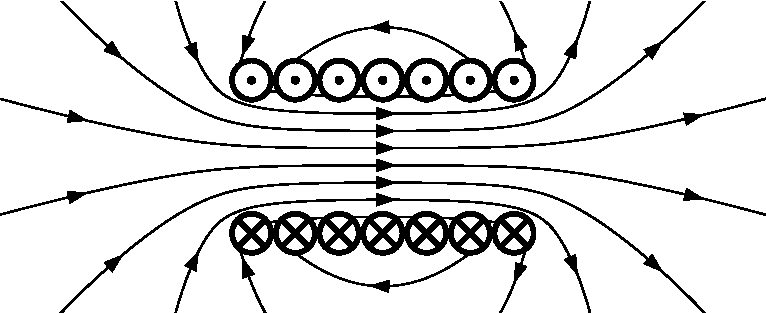
\includegraphics[width=0.5\textwidth]{solenoid.pdf}
\caption{\label{fig:solenoid1} A cross-sectional view of a solenoid.}
\end{figure}

\begin{enumerate}
\item Consider Fig. \ref{fig:solenoid1}.  Let the radius from the center of the solenoid to the outer edge be $R$.  The turns per unit length is $n = N/L$, where $N$ is the total number of tursn and $L$ is the length.  The current is $I$.  Prove that the B-field inside the solenoid is 
\begin{equation}
\vec{B} = \mu_0 n I\hat{x}
\end{equation}
The direction $\hat{x}$ is whichever direction is appropriate given the direction of the current (RHR-2). \\ \vspace{1cm}
\item Imagine a single circular loop of wire with radius $r$ inside the solenoid.  If a uniform E-field $\vec{E}$ along this loop exists, show that 
\begin{equation}
\oint \vec{E} \cdot d\vec{l} = 2\pi r E
\end{equation}
\vspace{1cm}
\item Supose the current $I$ started to shift: $I(t) = I_0 + bt$.  (a) What would be the induced electric field along the loop inside the solenoid? Is it a constant? (b) What would have to change in order to make the E-field depend on time? \\ \vspace{2cm}
\item Suppose for a brief moment that $a = 100$ A/s, and that $n = 1000$ turns per meter.  Let also the inner coil have $N = 100$ turns and a radius of $r = 1$ cm.  What is the induced E-field value?
\end{enumerate}
\end{document}
